\documentclass{article}

\usepackage{amsmath, amsthm, amssymb, amsfonts}
\usepackage{thmtools}
\usepackage{graphicx}
\usepackage{setspace}
\usepackage{geometry}
\usepackage{float}
\usepackage{hyperref}
\usepackage[utf8]{inputenc}
\usepackage[english]{babel}
\usepackage{framed}
\usepackage[dvipsnames]{xcolor}
\usepackage{environ}
\usepackage{tcolorbox}
\tcbuselibrary{theorems,skins}

% Commands
\newcommand{\lcm}{\operatorname{lcm}}
\newcommand{\bz}{\mathbb{Z}}
\newcommand{\bn}{\mathbb{N}}
\newcommand{\br}{\mathbb{R}}
\newcommand{\ibz}{\in \mathbb{Z}}
\newcommand{\ibn}{\in \mathbb{N}}
\newcommand{\ibr}{\in \mathbb{R}}

% Definition
\newtcbtheorem[number within=subsection]{mydefinition}{Definition}
{
    enhanced,
    frame hidden,
    titlerule=0mm,
    toptitle=1mm,
    bottomtitle=1mm,
    fonttitle=\bfseries\large,
    coltitle=black,
    colbacktitle=green!20!white,
    colback=green!10!white,
}{df}

\NewDocumentCommand{\defn}{m+m}{
    \begin{mydefinition}{#1}{}
        #2
    \end{mydefinition}
}

\NewDocumentCommand{\udefn}{m+m}{
    \begin{mydefinition*}{#1}{}
        #2
    \end{mydefinition*}
}

\setstretch{1.2}
\geometry{
    textheight=9in,
    textwidth=5.5in,
    top=1in,
    headheight=12pt,
    headsep=25pt,
    footskip=30pt
}

% Theorem
\newtcbtheorem[use counter from=mydefinition]{mytheorem}{Theorem}
{
    enhanced,
    frame hidden,
    titlerule=0mm,
    toptitle=1mm,
    bottomtitle=1mm,
    fonttitle=\bfseries\large,
    coltitle=black,
    colbacktitle=cyan!20!white,
    colback=cyan!10!white,
}{th}

\NewDocumentCommand{\thm}{m+m}{
    \begin{mytheorem}{#1}{}
        #2
    \end{mytheorem}
}

\NewDocumentCommand{\uthm}{m+m}{
    \begin{mytheorem*}{#1}{}
        #2
    \end{mytheorem*}
}

% Lemma
\newtcbtheorem[use counter from=mydefinition]{mylemma}{Lemma}
{
    enhanced,
    frame hidden,
    titlerule=0mm,
    toptitle=1mm,
    bottomtitle=1mm,
    fonttitle=\bfseries\large,
    coltitle=black,
    colbacktitle=violet!20!white,
    colback=violet!10!white,
}{lm}

\NewDocumentCommand{\lem}{m+m}{
    \begin{mylemma}{#1}{}
        #2
    \end{mylemma}
}

\NewDocumentCommand{\ulem}{m+m}{
    \begin{mylemma*}{#1}{}
        #2
    \end{mylemma*}
}

% Corollary
\newtcbtheorem[use counter from=mydefinition]{mycorollary}{Corollary}
{
    enhanced,
    frame hidden,
    titlerule=0mm,
    toptitle=1mm,
    bottomtitle=1mm,
    fonttitle=\bfseries\large,
    coltitle=black,
    colbacktitle=orange!20!white,
    colback=orange!10!white,
}{cl}

\NewDocumentCommand{\cor}{+m}{
    \begin{mycorollary}{#1}{}
        #1
    \end{mycorollary}
}

\NewDocumentCommand{\ucor}{+m}{
    \begin{mycorollary*}{}{}
        #1
    \end{mycorollary*}
}

% Proposition
\newtcbtheorem[use counter from=mydefinition]{myproposition}{Proposition}
{
    enhanced,
    frame hidden,
    titlerule=0mm,
    toptitle=1mm,
    bottomtitle=1mm,
    fonttitle=\bfseries\large,
    coltitle=black,
    colbacktitle=yellow!20!white,
    colback=yellow!10!white,
}{pr}

\NewDocumentCommand{\prop}{+m}{
    \begin{myproposition}{}{}
        #1
    \end{myproposition}
}

\NewDocumentCommand{\uprop}{+m}{
    \begin{myproposition*}{}{}
        #1
    \end{myproposition*}
}

% Claim
\newtcbtheorem[use counter from=mydefinition]{myclaim}{Claim}
{
    enhanced,
    frame hidden,
    titlerule=0mm,
    toptitle=1mm,
    bottomtitle=1mm,
    fonttitle=\bfseries\large,
    coltitle=black,
    colbacktitle=pink!20!white,
    colback=pink!10!white,
}{cl}

\NewDocumentCommand{\clm}{+m}{
    \begin{myclaim}{}{}
        #1
    \end{myclaim}
}

\NewDocumentCommand{\uclm}{+m}{
    \begin{myclaim*}{}{}
        #1
    \end{myclaim*}
}

% Proof
\NewDocumentCommand{\pf}{+m}{
    \begin{proof}
        [\hspace{1em}\textbf{Proof.}]
        #1
    \end{proof}
}



% ------------------------------------------------------------------------------

\begin{document}
\title{ \normalsize \textsc{}
		\\ [2.0cm]
		\LARGE \textbf{
        \LARGE{MATH 101} \vspace*{10\baselineskip}}
		}
\date{}
\author{\textbf{Professor} \\ 
		\LaTeX\:by Jack\\
		University \\
        Semester}

\maketitle
\newpage

\tableofcontents
\newpage

% ------------------------------------------------------------------------------

\section{Examples}

\udefn{Definition Name}{
    A defintion.
}

\uthm{Theorem Name}{
    A theorem.
}

\ulem{Lemma Name}{
    A lemma.
}

\ucor{
    A corollary.
}

\uprop{
    A proposition.
}

\uclm{
    A claim.
}

\pf{
    Veniam velit incididunt deserunt est proident consectetur non velit ipsum voluptate nulla quis. Ea ullamco consequat non ad amet cupidatat cupidatat aliquip tempor sint ea nisi elit dolore dolore. Amet sunt duis adipisicing ad esse aute officia laborum anim cupidatat sit adipisicing ea. Elit officia esse deserunt laborum sit ex commodo ad incididunt. Est occaecat culpa excepteur sunt esse consectetur ut elit elit officia ipsum officia nisi sint irure.

    Laboris labore magna dolore eiusmod ea ex et eiusmod laboris. Et aliquip cupidatat reprehenderit id officia pariatur. Pariatur dolore qui amet ad sit minim esse minim. Lorem cillum velit nisi pariatur qui reprehenderit consectetur nostrud est officia nostrud officia ex nostrud veniam.
}

\subsection{Pictures}

\begin{figure}[H]
    \center
    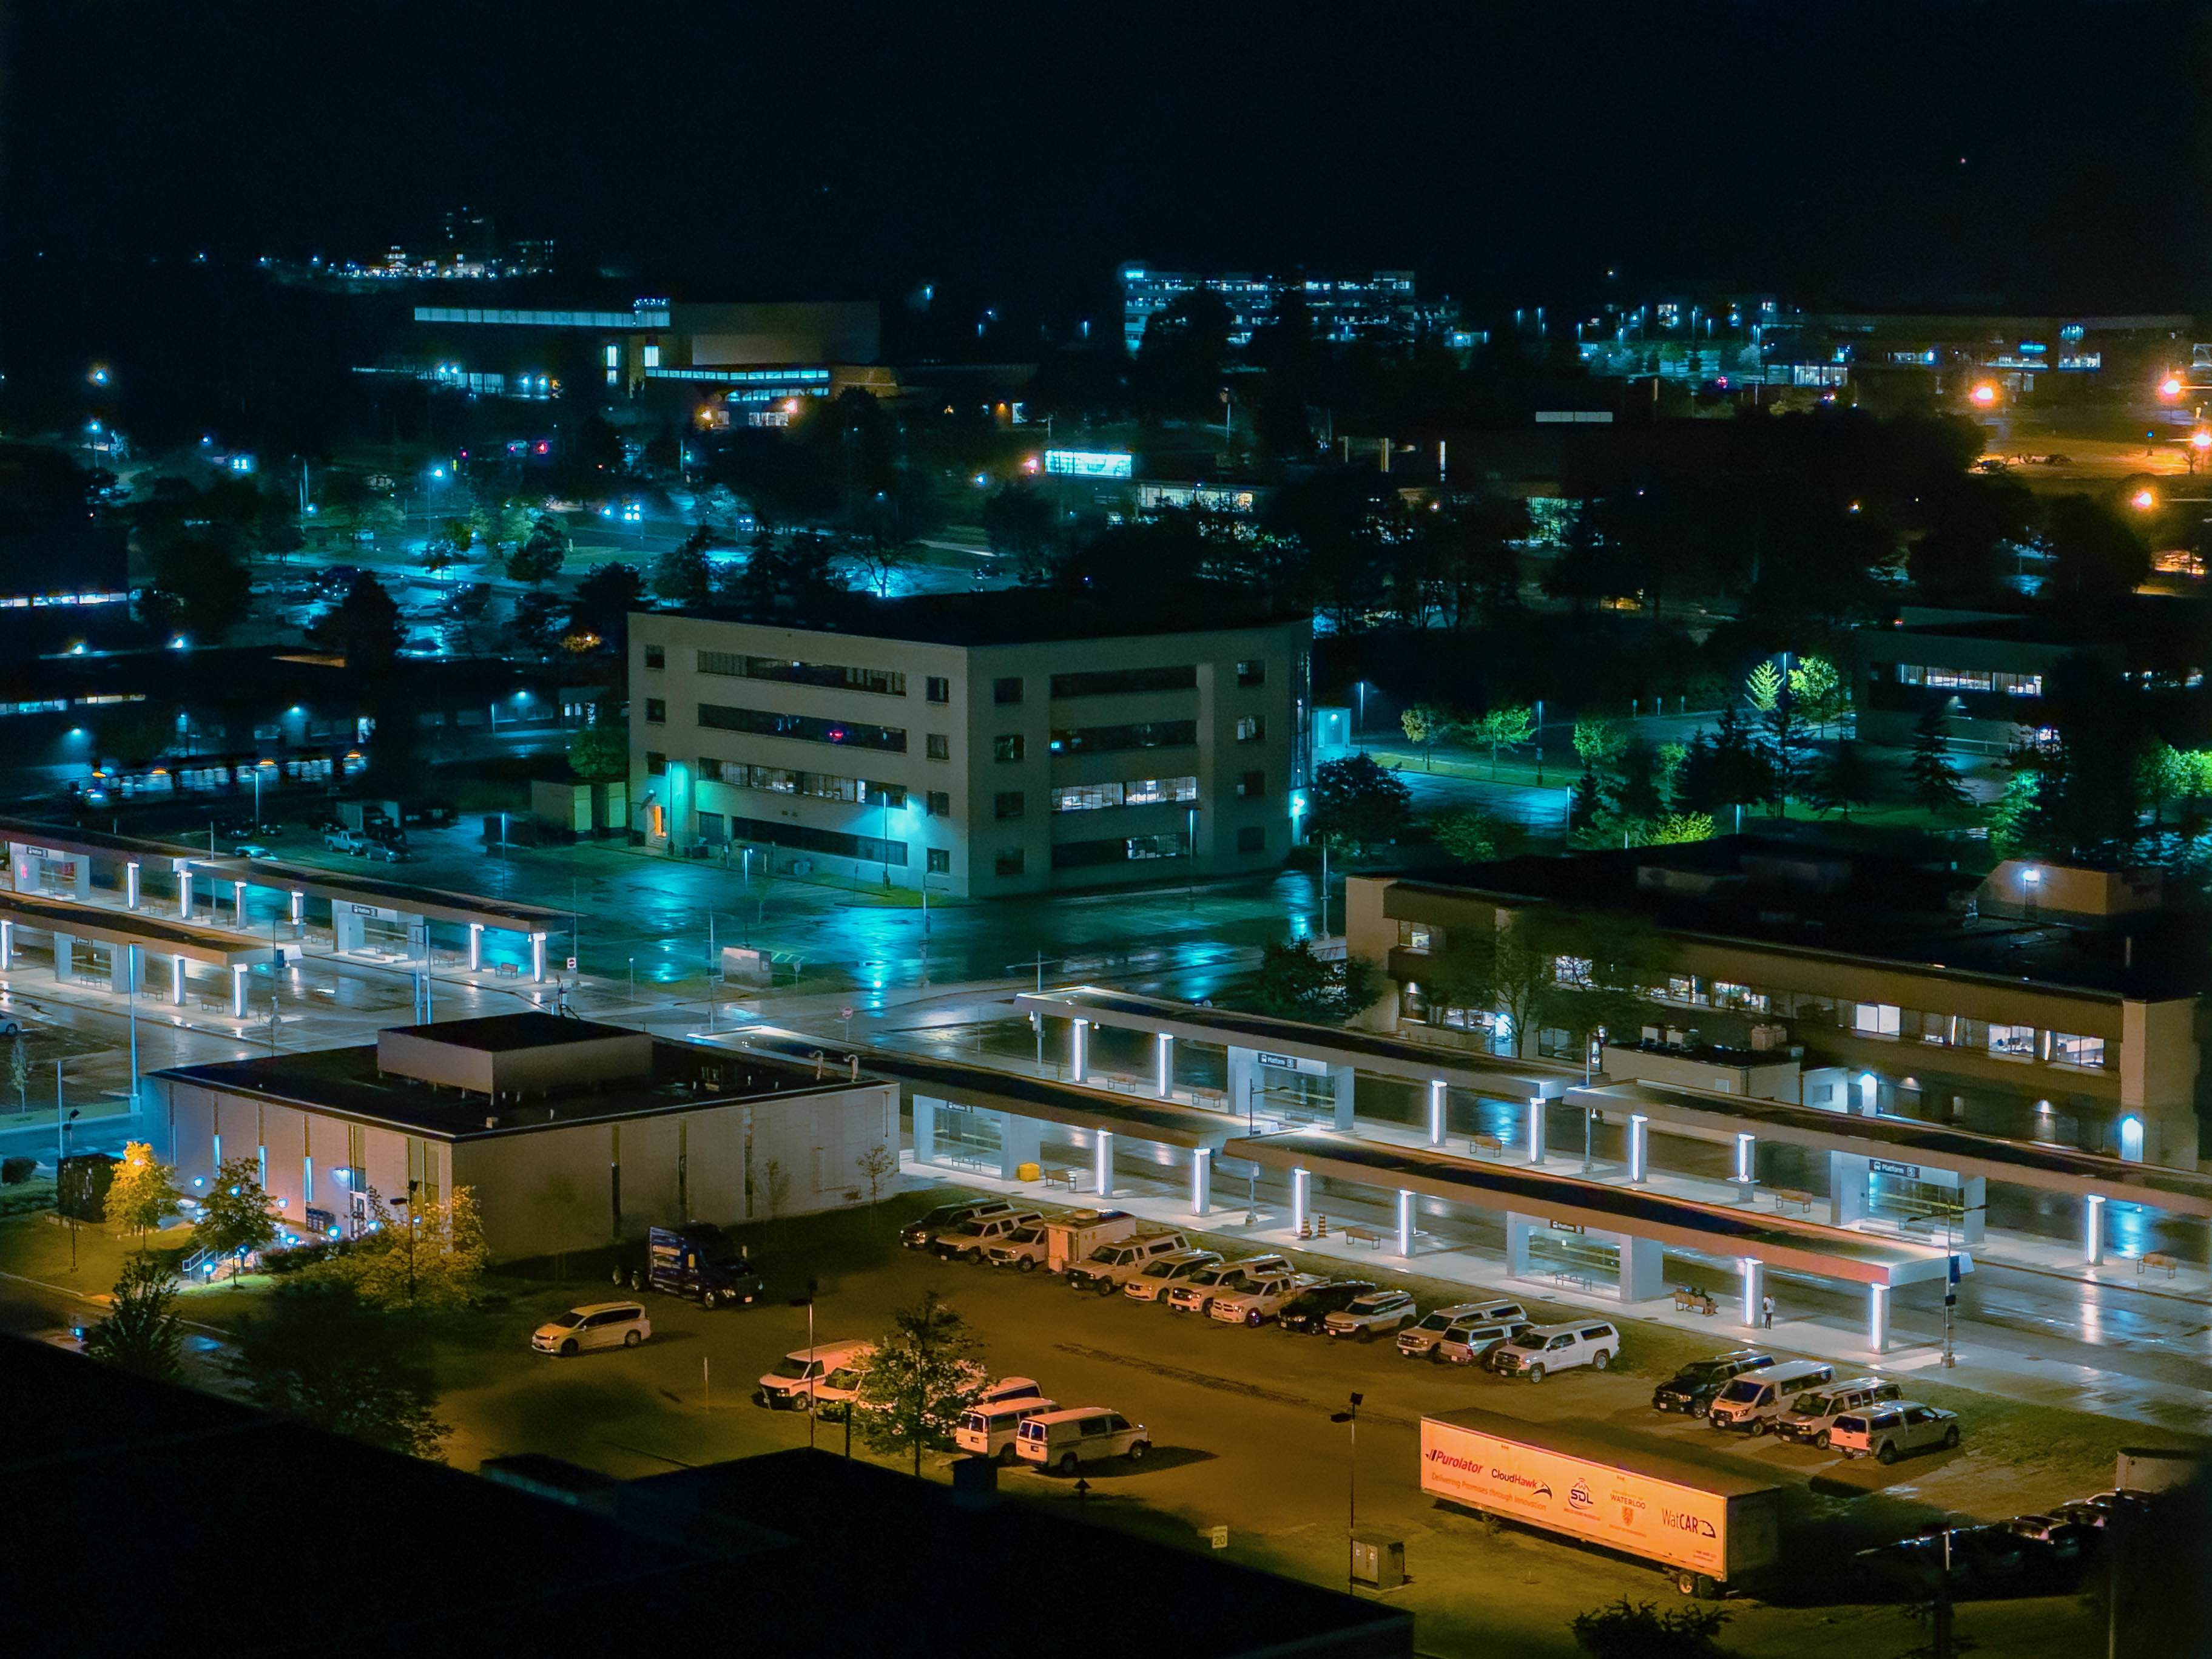
\includegraphics[scale=0.1]{img/loo.jpg}
    \caption{Waterloo, ON}
\end{figure}

\end{document}
